\documentclass[aspectratio=43]{beamer}
\usepackage[utf8]{inputenc}
\usepackage{beamer_eit-en}
\usepackage[document]{ragged2e}
\usepackage{lineno}
\usepackage{graphicx,wrapfig,lipsum}
\usepackage{sidecap}
\usepackage[english]{babel}
\usepackage[utf8]{inputenc}
\usepackage{amsmath}
\usepackage{siunitx}
\setbeamertemplate{caption}[numbered]

\begin{document}

\title[Scientific Working 2018  ]{\huge {Novel MRI Technique Enables Non-Invasive Measurement of Atrial Wall Thickness}}
\author{\small \justify {Arthor: Varela, M., Morgan, R., Theron, A., Dillon-Murphy, D., Chubb, H., Whitaker,J., Henningsson, M., Aljabar, P.,Schaeffter, T., Kolbitsch, C., and Aslanidi,
O. V. (2017).
IEEE Transactions on Medical Imaging, 36(8):1607–1614}}
 
\institute{
	{\large Presented by : Md Amir Hossain \\ Date : 01.06.2018
}}
\mode<presentation>{\keywords{Atrial Wall thickness ,atrial fibrillation,catheter ablation, atrial imaging, black-blood MRI; atrial atlas}}
\date[01.06.2018]



\begin{frame}
        \maketitle
        
\end{frame}
\section{Table of contents}
\begin{frame}{Table of contents}
\LARGE {
        \begin{itemize}
        \item Introduction
        \item Methods 
        \item Results
        \item Discussion
        \item Conclusion
        \item References
        \end{itemize}
        }
\end{frame}
\newpage


\section{Introduction}
\begin{frame}{Introduction}
\normalsize {
        \begin{itemize}
        \item Measuring thickness of thinner Atrial Wall is still a great challenge.
        \item This measurement of AWT(Atrial Wall Thickness) can provide vital information in diagnosing and treatment of various heart diseases for example : atrial arrhythmias[2] , atrial tachycardias (AT) and atrial fibrillation (AF). 
        \item 48\%-65\% patients suffers recurrence of AF due to insufficient energy delivery during catheter ablation[3] .AWT map could help to select optimal energy for catheter ablation .
        \item AWT can help to locate location of rotors to terminate AF completely. 
        \end{itemize}
        }
\end{frame}

\newpage
\begin{frame}{Introduction: Imaging }
\normalsize {
\begin{itemize}
\item Post-Mortem studies : Limited in spatial coverage ,dependent on direction of sectioning , provides variable estimation of AWT[3]
\item Computer Tomography (CT): Poor soft tissue contrast ,difficulty in detection of Atrial border.
\item MRI : Higher soft tissue contrast , High contrast between blood and myocardium. 
\item \textbf{In this Study : a 3D based phase-sensitive inversion recovery (PSIR) protocol is utilized to produce a high-resolution black-blood MR images to measure Atrail  wall thickness. }

\end{itemize}
}
\end{frame}

\newpage
\section{Methods}
\subsection{Process block diagram }

\begin{frame}{Methods}
\begin{figure}[h!]	
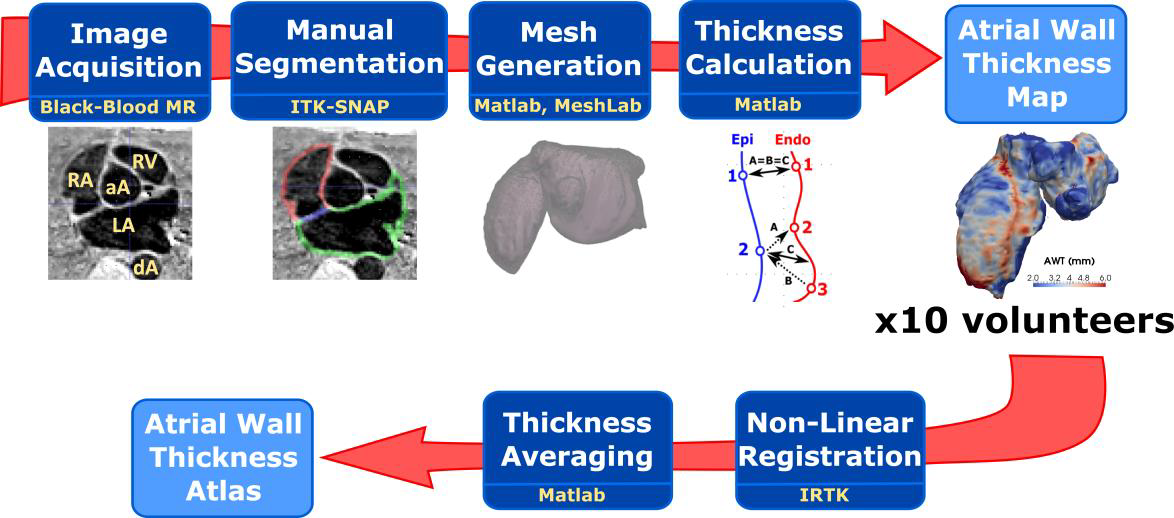
\includegraphics[width=\linewidth]{img/Pipeline}
\caption{Process to create Atrial wall thickness Map (see page 2,figure 1-Varela(2017))}
\label{Process to create Atrial wall thickness Map  }
\end{figure}
\end{frame}


\newpage
\subsection{Imaging of Volunteers}
\begin{frame}{Methods-Imaging of Volunteers}
\begin{minipage}{0.6\textwidth}\raggedleft
\begin{itemize}
        \item 10 healthy subject ( 3 female, 21-30 years old).
        \item Philips 3T Achieva scanner used. 
        \item Resolution : Image acquired in Para-axial plane using a PISR sequence with 3D flash(FOV),Flip angle:20 degree;repetition time 2.7/5.9 ms;SENSE factor: 1.5; fat suppression using SPIR.    
        \item Tigger delay(TD): 600-750 ms; depends on subjects heart rate.
        \item Real scan time: 13-23 min
\end{itemize}
\end{minipage}
\begin{minipage}{0.4\textwidth}\raggedleft
\begin{figure}


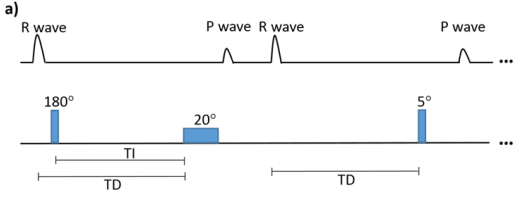
\includegraphics[width=\linewidth]{img/img1}

\caption {Pulse sequence diagram, over two cardiac cycles, of the PSIR sequence used in volunteers(page 3,figure 3-Varela(2017))}
\end{figure}
\end{minipage}

\noindent

\end{frame}

\newpage
\subsection{Imaging of Patients}
\begin{frame}{Methods-Imaging of Patients}
\begin{itemize}
\item AWT measured in the LA of 2 AF patients.
\item Only data of left atrial was measured .
\item 1.5T  Achieva scanner used ,Real scan time: 9-15min.
\item Image resolution as volunteer scans.
\item Data scaned immediately prior to ventricular relaxation .
\begin{figure}[h!]
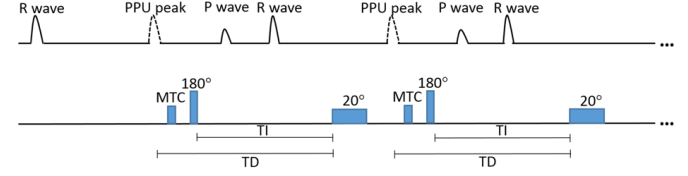
\includegraphics[width=\linewidth]{img/img2}
\caption{Pluse sequence diagram,over two cardiac cycle, of the sequence used in patients.(page 3,figure 3-Varela(2017))}
\end{figure}
\end{itemize}
\end{frame}

\newpage
\subsection{Table: PATIENT SCANS}
\begin{frame}{Methods-Table: PATIENT SCANS}


\begin{table} 
\begin{center}
  \begin{tabular}{c c c p{4cm} c}
    \hline
     Number& Age & Gender & Clinical Details & LA AWT (mm) \\ \hline
     
    \hline
    1 & 32 & M & Paroxysmal AF \newline prosthetic (tissue) mitral valve replacement, 1 previous surgical ablation, 2 previous catheter ablations & \begin{math}
    3.1\pm1.3
\end{math}
\\ \hline
2 & 74 & F & Paroxysmal AF, hypertension, 1 previous cardioversion, no previous ablations & \begin{math}
    2.6\pm 0.7
\end{math} 
\\ \hline \hline


  \end{tabular}
  \caption{Clinical details of the two scanned patients, accompanied by the obtained atrial wall thickness values in the left atrium. (Varela(2017))}
 

\end{center}
 \end{table}
 \end{frame}
 
 \newpage
 \subsection{Image processing}
 \begin{frame}{Methods- Image processing}
 \begin{itemize}
 \item Surfaces of Atrial epicardial and endocardial were segmented manually using 4 individual operator using ITK-SNAP and Seg3D.
 \item When it was not possible to indicate the border between the LA wall and the arotic root wall ,the complete border of LA wall and arotic root was included.
 \item The segmentation of entire atria was performed mainly by segmenting along consecutive axial planes.
 \item Istropic Gaussian \begin{math}( \sigma = 0.2 voxels)\end{math} smoothing was performed to decrease sharp edge between different axial planes.
 \item The segmentation of the LA of 4 random variables (2 volunteers and 2 patients) blindly repeated to gauge the  reproducibility of the segmentation.
   
 \end{itemize}
 
 \end{frame}
 
 \newpage
\subsection{Thickness Measurement} 
 
 \begin{frame}{Methods-Thickness Measurement}
\begin{minipage}{0.8\textwidth}\raggedleft
\begin{itemize}
        \item By using marching cubes algorithm ,triangular meshes of each of the atrial surface were generated in Mathlab.
        \item AWT was measured by the average of nearest neighbours Method : A) measuring the distance between each node in the epicardial surface and its nearest neighbor in the endocardial surface; B) repeating procedure A) in reverse for each node in the endocardial wall; C) averaging the outcomes of procedures A) and B).   
        \item AWT was encoded as a scalar field mapped to each vertex in the epicardial mesh.
        \item For vessel openings and the mitral and tricuspid valves, the nominal AWT was set to 0.
     
\end{itemize}
\end{minipage}
\begin{minipage}{0.2\textwidth}\raggedleft
\begin{figure}[h!]


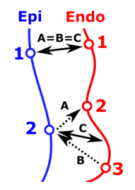
\includegraphics[width=\linewidth]{img/img3}

\caption {The average of nearest neighbors method for measuring AWT.(Varela(2017))}
\end{figure}
\end{minipage}

\noindent


\newpage
\subsection{Impact of Acquisition Resolution}
\end{frame}
 
 \begin{frame}{Methods- Impact of Acquisition Resolution}
 \begin{itemize}
 \item Imaging done of 2 volunteers at a higher resolution of 1.0mm to determine if image acquisition resolution introduce a bias in AWT estimation.
 \item Average of nearest method was used to measure the AWT of the widely used visible Female atrial geometry ( segmentation of 0.33mm resolution picture of Cryosections of a female cadaver)[4].
 \item Cryosections provides reconstruction of every fine details of the cardiac anatomy .
 \item Compared AWT estimated using this database and the obtained MR image as a further test for the impact of the acquisition resolution on AWT estimates.
 \end{itemize}
 
 \end{frame}
 
\newpage
\subsection{ Atlas Creation} 
\begin{frame}{Methods- Atlas Creation}
\begin{itemize}
\item Epicardial meshes from all volunteers were manually aligned.
\item Non-linearly registered to the reconstructed atrial surface using visual inspection.
\item The registration was done with the snreg tool of the Image Registration Toolkit.
\item For each vertex of the target image, AWT was measured by averaging the AWT values in the matching vertices of the epicardial meshes of each of the imaged subjects using Matlab.
\item The uncertainty in AWT measurement was estimated, on a vertex-by-vertex basis, using the standard deviation of AWT across all subjects.
\item Patient scans were not used as inputs to the AWT atlas.

\end{itemize}

\end{frame}

\newpage
\section{Results}
\subsection{Imaging and Atrial wall thickness Maps}
\begin{frame}{Results- Imaging and Atrial wall thickness Maps}
\begin{minipage}{0.5\textwidth}\raggedleft
\begin{itemize}

\item Three orthogonal representation from typical PSIR images with Atrial wall segmentation.
        \item Blood has a very low intensity, whereas myocardium appears hyperintense .
          
        \item Clearly distinguishable from both blood and surrounding non-cardiac tissue.
        
\end{itemize}
\end{minipage}
\begin{minipage}{0.5\textwidth}\raggedleft
\begin{figure}[h!]


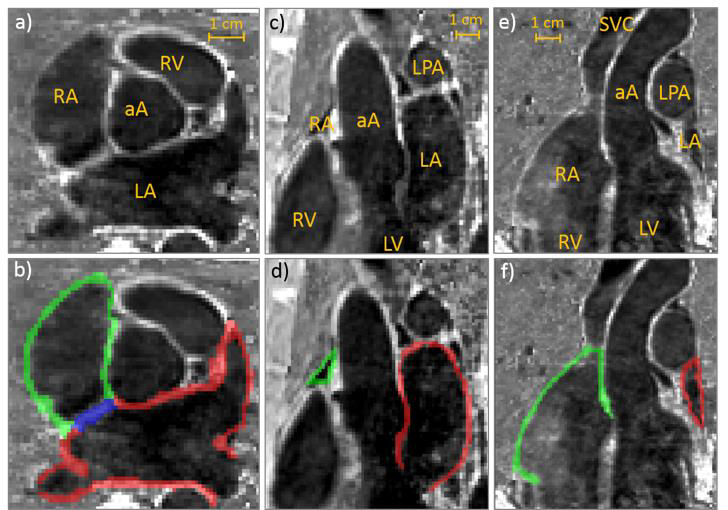
\includegraphics[width=\linewidth]{img/img4}

\caption {a, b) Axial, c, d) sagittal and e, f) coronal views of the atria from one representative subject overlaid.(page 4,Fig.3(Varela(2017))}
\end{figure}
\end{minipage}

\noindent



\end{frame}

\newpage
\subsection{Atrial wall thickness in Patients}
\begin{frame}{Results- Atrial wall thickness in Patients}
\begin{minipage}{0.5\textwidth}\raggedleft
\begin{itemize}
        \item AWT maps of LA of the two different diagnosed patients.
          \item AWT value in the left atrium : 3.1\begin{math}\pm \end{math} 1.3 mm .
        \item The AWT values for patient 2 are similar to those obtained in volunteers.
        \item patient 1 suffered from mitral regurgitation and enlarged left atrial cavity,lead increased left atrial AWT.
        
\end{itemize}
\end{minipage}
\begin{minipage}{0.4\textwidth}\raggedleft
\begin{figure}[h!]


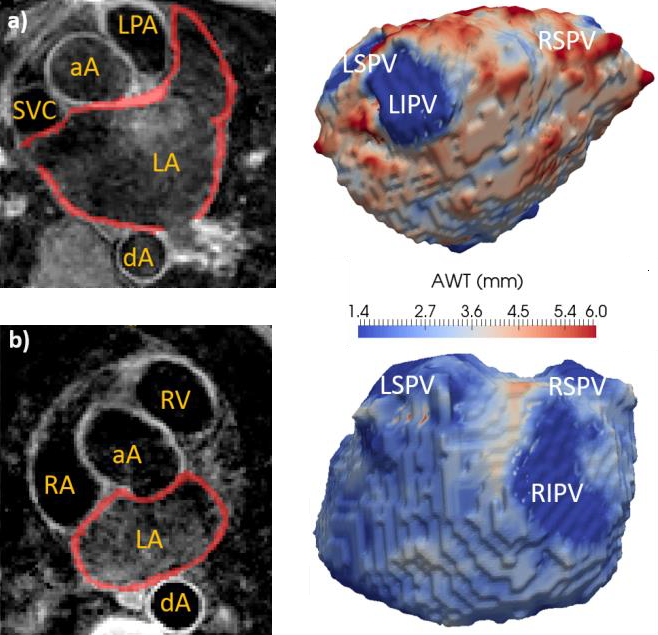
\includegraphics[width=\linewidth]{img/img5}

\caption {Left atrial axial view overlaid with the performed manual segmentations for: a) patient 1 and b) patient 2 .(page 4,Fig.4(Varela(2017))}
\end{figure}
\end{minipage}

\noindent



\end{frame}

\newpage
\subsection{Atrial wall thickness in subjects}
\begin{frame}{Results- Atrial wall thickness in subjects}
\begin{minipage}{0.6\textwidth}\raggedleft
\begin{itemize}
        \item AWT maps of LA of the two different diagnosed volunteers.
          \item A high tickness in the terminal crest(TC) region and low AWT in the pulmonary vein (PV) sleeves can be observed.
        \item The The Dice coefficient for the segmentation of the LA of the 4 analyzed subjects : 0.68mm \begin{math}\pm \end{math}0.06mm .
        \item The 50\%-percentile modified Hausdorff distance : 0.7mm \begin{math}\pm \end{math}0.2 mm.
        
\end{itemize}
\end{minipage}
\begin{minipage}{0.4\textwidth}\raggedleft
\begin{figure}[h!]


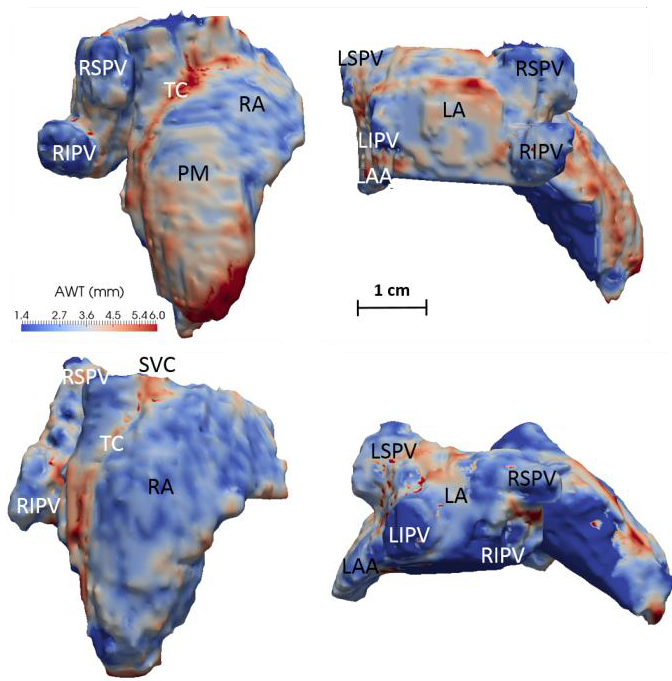
\includegraphics[width=\linewidth]{img/img6}

\caption {Atrial thickness of the LA and RA of two volunteers. (page: 5,Fig.5(Varela(2017)) }
\end{figure}
\end{minipage}

\noindent



\end{frame}



\newpage
\subsection{Atrial wall thickness Atlas}
\begin{frame}{Results- Atrial wall thickness Atlas}
\begin{minipage}{0.6\textwidth}\raggedleft
\begin{itemize}
        \item AWT map of the 10 volunteers.
          \item Both side of Atria have similar average thickness :2.7 \begin{math}\pm \end{math} 0.7 mm.
                \item Little variation of thickness(<0.1 mm) observed in different subject.
        \item The terminal crest thickness : 3.5 \begin{math}\pm \end{math} 4.2 mm.
        \item The pulmonary veins thickness : 1.5 \begin{math}\pm \end{math} 2.2 mm ,thinner than atrial wall.
        
\end{itemize}
\end{minipage}
\begin{minipage}{0.4\textwidth}\raggedleft
\begin{figure}[h!]


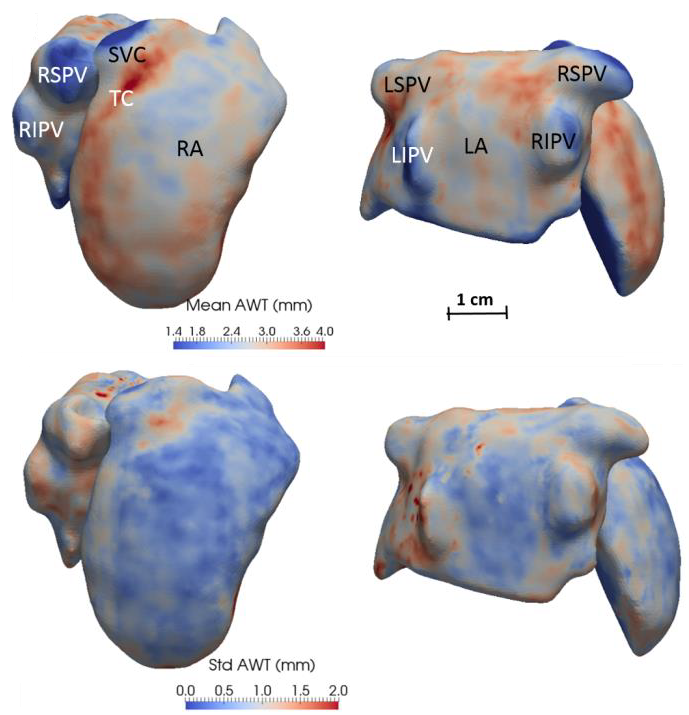
\includegraphics[width=\linewidth]{img/img7}

\caption {Atrial thickness created from 10 healthy volunteers. (page: 5,Fig.6(Varela(2017)) }
\end{figure}
\end{minipage}

\noindent



\end{frame}

\newpage


\subsection{Comparison with Literature}
\begin{frame}{Results-Comparison with Literature}
\begin{minipage}{0.88\textwidth}
\begin{figure}[h!]
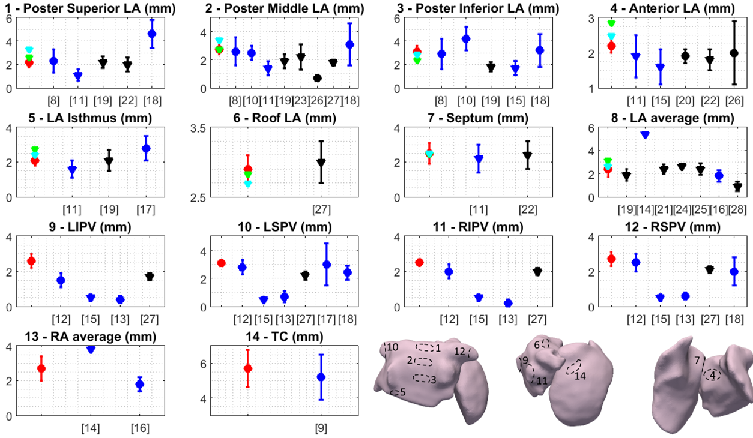
\includegraphics[width=\linewidth]{img/img8}\centering 
\caption{\scriptsize AWT measured in several regions in MRI in volunteers (red), Patient 1 (green) and Patient 2 (light blue),literature measurements using CT (black).(Page:6, Fig.7 Varela(2017)) }

\end{figure}
\end{minipage}

\end{frame}

\newpage

\begin{frame}{Results-Comparison with Literature cont.}
\begin{itemize}
\item The measured AWT are in general in good agreement with studies using other modalities.
\item The posterior left atrial wall,for ablation procedures was thicker in its inferior region, as same in the post-mortem literature.
\item The thickness of the PVs were performed approximately 0.5 cm away from the ostia, to match previous studies[7]. 
\item In the RA, AWT has been measured in fewer specific regions, the exception being the terminal crest,the thickest region of the atria, matches post-mortem reports.

\end{itemize}
\end{frame}

\newpage
\subsection{Impact of Acquisition Resolution}
\begin{frame}{ Results- Impact of Acquisition Resolution}
\begin{itemize}
\item For one volunteer, the 1.0mm resolution was unsuccessful due to low breathing efficiency. 
\item The measured AWT in higher resolution was 2.9mm\begin{math} \pm \end{math} 1.1 mm, and 3.3mm \begin{math} \pm \end{math} 1.2mm obtained using the lower resolution scan in the same cooperative volunteer.
\item The AWT of the Visible Female atrial model: 2.7mm \begin{math} \pm \end{math} 1.4 mm, with high resolution: 2.4mm \begin{math} \pm \end{math} 0.8 mm.

\end{itemize}

\end{frame}

\newpage
\section{Discussion}
\begin{frame}{Discussion}
\begin{itemize}
\item A novel contrast agent-free MRI protocol is used to obtain AWT information in a 10-min free-breathing scan.
\item Creation of the first whole atria atlas of wall thickness from images of 10 healthy volunteers.
\item Atrial wall thickness maps in 2 AF patients.

\end{itemize}
\textbf{A. Image Acquisition and Processing}
\begin{itemize}
\item The acquired images show a good contrast between the atrial myocardium, blood and periatrial structures.
\item The endo- and epicardial surfaces were manually segmented.
\item Automatic segmentation is considerably harder to implement in MRI than in CT.
\item Further studies will explore the use of automatic segmentation techniques.
\end{itemize}
\end{frame}
\begin{frame}{Discussion}
\textbf{B. Atrial Wall Thickness Measurements}
\begin{itemize}
\item AWT computed using average of nearest neighbors method.
\item This computation method was used cortical thickness measurement.
\item A 1.40-mm isotropic resolution used as a balance between spatial resolution, signal to noise ratio and scan time.
\item imaging in a very long scan, the atria of a cooperative volunteer possible at a higher resolution of 1.0 mm.
\item AWT values were comparable, shows spatial resolution didn't create systematic errors in AWT measurement.
\item Future research will explore the impact of imaging resolution on AWT measurements more quantitatively. 
\end{itemize}
\end{frame}

\newpage
\begin{frame}{Discussion}
\textbf{C. Atrial Wall Thickness Atlas}
\begin{itemize}
\item AWT atlas was created by non-linear registration of 10 volunteer AWT maps.
\item Measured thickness values matches with previous literature reports from post-mortem and CT studies.
\item The volunteer AWT atlas can provide important information about computational studies of atrial fibrillation.
\item The atlas can help to identify  atrial wall thickness roles in the dynamics and location of the abnormal electrical circuits underlying AF.
\item The atlas can also be utilize for future studies to determine how disease, age or medical interventions can affect AWT.
\end{itemize}
\end{frame}

\newpage
\begin{frame}{Discussion}
\textbf{D. Atrial Wall Thickness in Patients}
\begin{itemize}
\item Successful implementation to image AF patients with sinus rhythm during scan.
\item The patient without structural heart disease had an AWT was similar to that of volunteers.
\item Patient showing notable differences in AWT,is higher than in the imaged volunteers.
\item The AWT maps and atlas can be utilize for modelling atrial electrophysiology and mechanics.
\item Due to insufficient inversion times to acquire improved blood-myocardium contrast,the high success rate in patients who are in AF is unlikely . 
\end{itemize}
\end{frame}


\newpage
\section{Conclusion}
\begin{frame}{Conclusion}
\begin{itemize}
\item A black-blood PSIR protocol used to measure atrial wall thickness maps in 10 healthy volunteers. 
\item The first wall thickness atlas for the entire atria measured by combining AWT maps.
\item Measured AWT estimates matches with other modalities.
\item the proposed scan can be easily utilize in the current clinical MRI protocols to create subject-specific AWT maps.
 \item Patients with progressive heart disease in the pre-ablation setting can be highly benefited by this technique. 
 \item This AWT information could provide vital information for both patient stratification and procedure like catheter ablation.
 
\end{itemize}
\end{frame}

\newpage
\section{References}
\begin{frame}{References}
\begin{enumerate}\scriptsize
\item Marta Varela, M., Morgan, R., Theron, A., Dillon-Murphy, D., Chub
b, H., Whitaker,J., Henningsson, M., Aljabar, P., Schaeffter, T., Kolbitsch, C., and Aslanidi,O. V. (2017). Novel MRI technique enables non-invasive measurement of atrial wall thickness.IEEE Transactions on Medical Imaging, 36(8):1607–1614
\item J. Whitaker, R. Rajani, H. Chubb, M. Gabrawi, M. Varela, M. Wright, S. Niederer, and M. O’Neill, “The role of myocardial wall thickness in atrial arrhythmogenesis,” Europace, vol. i, no. 7, p. euw014, May 2016
\item D. Sánchez-Quintana, R. H. Anderson, J. a Cabrera, V. Climent, R. Martin, J. Farré, and S. Y. Ho, “The terminal crest: morphological features relevant to electrophysiology.,” Heart, vol. 88, no. 4, pp. 406–411, Oct. 2002
\item M. J. Ackerman, “The Visible Human Project,” Proc. IEEE, vol. 86, no. 3, pp. 504–511, Mar. 1998.
\item P. G. Platonov, V. Ivanov, S. Y. Ho, and L. Mitrofanova, “Left atrial posterior wall thickness in patients with and without atrial fibrillation: data from 298 consecutive autopsies.,” J. Cardiovasc. Electrophysiol., vol. 19, no. 7, pp. 689–92, Jul. 2008.

\end{enumerate}
\end{frame}


\begin{frame}{}
  \centering \LARGE
  \emph{Thank you for your attention!}
\end{frame}
\end{document}